\documentclass[11pt]{extarticle}
\usepackage{apacite, setspace}
\usepackage[margin=1in]{geometry}
%\usepackage{times}
\usepackage{setspace}
\usepackage{float}
\usepackage{subfig}
\usepackage{tikz}
\usepackage{titlesec}
\usepackage{booktabs} % To thicken table lines
\usepackage[shortlabels]{enumitem}
\usepackage{amsthm,amssymb} % for proof 
\usepackage[bottom]{footmisc} %footnote to bottom
\usepackage{amsmath}



\usepackage{amsfonts}
% image
\usepackage{graphicx}
\graphicspath{ {img/} }

\usepackage{array}
\newcolumntype{L}[1]{>{\raggedright\let\newline\\\arraybackslash\hspace{0pt}}m{#1}}
\newcolumntype{C}[1]{>{\centering\let\newline\\\arraybackslash\hspace{0pt}}m{#1}}
\newcolumntype{R}[1]{>{\raggedleft\let\newline\\\arraybackslash\hspace{0pt}}m{#1}}


\titlespacing*{\section}
{0pt}{0px}{0px}


% image
\usepackage{graphicx}
\graphicspath{ {img/} }

% for header
\usepackage{fancyhdr}
\pagestyle{fancy}
\lhead{\textbf{ELEC 321 -- Stochastic Signals \& Systems: Homework 1}}
\rhead{Charles Clayton \texttt{\#21518139} \thepage}
\cfoot{}
\renewcommand{\headrulewidth}{0.4pt}
\renewcommand{\footrulewidth}{0.4pt}
 
% for indenting verbating
\usepackage{fancyvrb}

\setlength{\parskip}{\baselineskip}

% automatically convert "" to ``''
\usepackage [autostyle, english = american]{csquotes}
\MakeOuterQuote{"}

\begin{document}

\pagenumbering{gobble}
\singlespacing



\subsubsection*{Problem 1}

\begin{enumerate}[(a)] 
\item $A \cap \overline{B} \cap \overline{C}$
\item $A \cap B \cap \overline{C}$
\item $A \cup B \cup C$
\item $(A \cap B) \cup (A \cap C) \cup (B \cap C)$
\item $A \cap B \	cap C$
\item $\overline{A} \cap \overline{B} \cap \overline{C}$
\item $(A \cap \overline{B} \cap \overline{C}) \cup (\overline{A} \cap B \cap \overline{C}) \cup (\overline{A} \cap \overline{B} \cap C)$
\item $ \overline{A} \cup \overline{B} \cup \overline{C} $
\item $(A \cap B \cap \overline{C}) \cup (A \cap \overline{B} \cap C) \cup (\overline{A} \cap B \cap C) $
\item $ \Omega $
\end{enumerate}

\subsubsection*{Problem 2}

\begin{enumerate}[(a)]
\item By Bonferroni's inequality: $$ P(A \cap B) \geq P(A) + P(B) - 1 =  0.9 + 0.8 - 1 = \textbf{0.7} $$
\item By the addition rule\footnote{Proved in class slide 10/16}: $$P(A \cap B) = P(A) + P(B) - P(A \cup B)$$

Since $P(A \cup B) \leq 1$, then $P(A \cap B) \geq P(A) + P(B) - 1 $

\item \begin{proof}[Proof] Consider the base case, $n=2$:
$$P(A_1 \cap A_2) \geq P(A_1) + P(A_2) - (2-1) = P(A_1) + P(A_2) - 1$$
Substituting $ P(A_1 \cap A_2) + P(A_1 \cup A_2) = P(A_1) + P(A_2) $ from the addition rule, we get:
$$P(A_1 \cap A_2) \geq P(A_1 \cap A_2) + P(A_1 \cup A_2) - 1$$
Since $P(A_1 \cup A_2) \leq 1$, then $P(A_1 \cup A_2) - 1 \leq 0$. Thus the inequality is true.

Induction hypothesis, for $k \in \mathbb{N}$: $$P(A_1 \cap A_2 \cap \dots \cap A_k) \geq P(A_1) + P(A_2) + \dots + P(A_k) - (k-1)$$
For $k+1$: $P(A_1 \cap A_2 \cap \dots \cap A_{k+1}) \geq P(A_1 \cap A_2 \cap \dots \cap A_{k}) + P(A_{k+1}) - 1 $
 
Substituting $P(A_1 \cap A_2 \cap \dots \cap A_{k})$ from our hypothesis: $$P(A_1 \cap A_2 \cap \dots \cap A_{k+1})  \geq P(A_1) + P(A_2) + \dots + P(A_k) - (k-1) + P(A_{k+1}) - 1 $$
And so:
$$P(A_1 \cap A_2 \cap \dots \cap A_{k+1})  \geq P(A_1) + P(A_2) + \dots + P(A_k) +  P(A_{k+1}) - \big( (k+1) - 1 \big) $$


\end{proof}

\item \begin{proof}[Proof]

Consider the base case, $n=2$. By the inclusion-exclusion principle:
$$P(\cup_{i=1}^2 A_i) = P(A_1 \cup A_2) = P(A_1) + P(A_2) - P(A_1 \cap A_2)$$
Since $P(A_1 \cap A_2) \geq 0$, then  $$P(\cup_{i=1}^2 A_i) \leq P(A_1) + P(A_2) 
 = \sum_{i=1}^{2} P(A_i)$$
Induction hypothesis, for $k \in \mathbb{N}$: $$P(\cup_{i=1}^k A_i) \leq \sum_{i=1}^{k} P(A_i)$$
For $k+1$, by the inclusion-exclusion principle:
$$P ( \cup_{i=1}^{k+1} A_i ) = P ( \cup_{i=1}^{k} A_i) + P(A_{k+1}) - P \big( A_{k+1} \cap  (\cup_{i=1}^{k} A_i) \big)$$
Since $P \big( A_{k+1} \cap  (\cup_{i=1}^{k} A_i) \big) \geq 0$, then:
$$P ( \cup_{i=1}^{k+1} A_i ) \leq P ( \cup_{i=1}^{k} A_i) + P(A_{k+1})$$
By our hypothesis:
$$P ( \cup_{i=1}^{k+1} A_i ) \leq \sum_{i=1}^{k} P(A_i) + P(A_{k+1}) = \sum_{i=1}^{k+1} P(A_i)$$
\end{proof}
\end{enumerate}


\subsubsection*{Problem 3 (Total Probability)}

\begin{proof}[Proof]

If $A_1, A_2, \dots A_n$ is a partition, then the entire sample space is accounted for ($\cup_{i=1}^n A_i = \Omega $) and all sets $A_1, A_2, \dots A_n$ are disjoint. 

Since $B \subseteq A_i$ for $i \in \mathbb{N}$, by the the \textit{Intersection of a Subset} theorem, $B = B \cap A_i$. Therefore:
$$P(B) = P \Big( B \cap \left( A_1 \cup A_2 \cup \dots \cup A_n \right) \Big)$$
By the distributive property:
$$P \Big( B \cap \left( A_1 \cup A_2 \cup \dots \cup A_n \right) \Big) = P \Big( (B \cap A_1) \cup (B \cap A_2) \cup \dots \cup (B \cap A_n)   \Big)$$
Since all $A_i$ are disjoint, then all  $ B \cap A_i$ are also disjoint. So by probability axiom three:
$$P \Big( (B \cap A_1) \cup (B \cap A_2) \cup \dots \cup (B \cap A_n)   \Big) = \sum_{i=1}^{n} P(A_i \cap B)$$

$P(B | A_i)$ indicates the probability of $B$ given $A_i$. By the \textit{conditional probability definition}: $$P(B | A_i) = \frac{P(B \cap A_i)}{P(A_i)} $$
Therefore: $$ \sum_{i=1}^{n} P(A_i \cap B) = \sum_{i=1}^{n}  P(B | A_i) P(A_i)$$
\end{proof}

\subsubsection*{Problem 4}

%Number of places for broken antenna is those between others, so $n-m+1$.

%Number of arrangements is : $${n-m+1 \choose m}$$




\begin{enumerate}[(a)]

\item For $n$ antennae, the number of linear orderings without consecutive antennas down is equal to the the $(n+1)$th element of the fibbonaci sequence, that is:

$$
\sum_{m=0}^{n} {n - m + 1 \choose m}
$$

\begin{table}[ht!]
\centering
\scriptsize
\begin{tabular}{c|ll}
\toprule
 &  & \textbf{\ \ \ \# orderings}  \\
\midrule
$\mathbf{n}$ & \textbf{total} & \textbf{w/o consecutive failures} \\
\midrule
0&1&1\\
1&2&2\\
2&4&3\\
3&8&5\\
4&16&8\\
5&32&13\\
6&64&21\\
7&128&34\\
8&256&55\\
9&512&89\\
10&1024&144\\
11&2048&233\\
12&4096&377\\
13&8192&610\\
14&16384&987\\
15&32768&1597\\
16&65536&2584\\
17&131072&4181\\
18&262144&6765\\
19&524288&10946 \\
\bottomrule
\end{tabular}
\normalsize
\end{table}

I determined this through simulation using the following Python code: 

\scriptsize
\begin{verbatim}

def binary_list(num, bits):
    u = format(num, "0" + str(bits) + "b")
    return [int(d) for d in u] 

def binary_list_sequence(bits):
    l = []
    for i in range(0, 2**(bits)):
        l.append(binary_list(i, bits))
    return l

def consecutive_zeros(l):
    for i in range(len(l) - 1):
        if(l[i] == 0 and l[i+1] == 0):
            return True
    return False

def number_with_consecutive_zeros(bits):
    nf = 0
    for l in binary_list_sequence(bits):
        if(not consecutive_zeros(l)): nf += 1
    return nf
 
for i in range(0, 20):
    print(i, "\t", 2**i, "\t", number_with_consecutive_zeros(i))
\end{verbatim}
\normalsize


\item Since $\sum_{i=0}^6 P(m=i) = 1$, the probability $P(m=6)$, $P(m=7) \dots P(m=10)=0$.

The probability that communication flows through the system is the probability that no two consecutive antennas are down: $$P = \frac{\#\text{ arrangements without consequtive failures}}{\#\text{ all possible orderings}}$$
$$ P(B) = \sum_{i=1}^{n}  P(B | A_i) P(A_i) $$ 
$$= P(B|A_1)P(A_1) +  P(B|A_2)P(A_2) +  P(B|A_3)P(A_3) + \dots +  P(B|A_{6})P(A_{6})$$ 
$$= \frac{1}{1} (0.11) + \frac{2}{2} (0.27) + \frac{3}{4}(0.30) +  \frac{5}{8} (0.20) + \frac{8}{16}  (0.09) + \frac{13}{32}  (0.02) +  \frac{21}{64} (0.01) = \textbf{0.68741}$$ 




%$$= \sum_{i=1}^{n} P(B \cap A_i) $$

%$$\frac{{n - m + 1 \choose m}}{\Omega}$$

\end{enumerate}


\subsubsection*{Problem 5}

\begin{enumerate}[(a)]

\item \begin{proof}[Proof] Suppose to the contrary that all points in the sample space are equally likely, such that $p_1, p_2, p_3 \dots p_\infty$ are all equal to some probability $\epsilon$. Then the sum of each point's probability would have to add up to 1\footnote{Where's this from}. However for \textit{case 1}, $\epsilon = 0$, then: $$ \sum_{i=1}^{\infty} p_i = \sum_{i=1}^{\infty} \epsilon = 0$$
Alternatively for \textit{case 2}, $\epsilon > 0$, then: $$ \sum_{i=1}^{\infty} p_i = \sum_{i=1}^{\infty} \epsilon = \infty$$.
Either way, $ \sum_{i=1}^{\infty} p_i \neq 1 $, therefore not all points are equally likely.
\end{proof}

\item Although all points cannot be equally likely, all points can have a positive probability so long as they converge. Consider the series:

$$ \sum_{i=1}^{\infty} \frac{1}{2^i} = 1$$

If $p_i = \frac{1}{2^i}$, then each $p_1, p_2, p_3 \dots p_{\infty}$ $ > 0 $ and $ \sum_{i=1}^{\infty} p_i = 1 $, as required. Therefore yes, all the points can have a positive probability of occuring.

For another example, consider the tutorial example 1.10

\end{enumerate}


\clearpage 
\subsubsection*{Problem 6}

\begin{enumerate}[(a)]

\item I argue this formula based on my experimental results from the following Python\footnote{Rewrite as R if time} code. This script generates all the possible combinations of $0$ and $1$ of $n$ bits, using a binary sequence. Respectively, these representing $heads$, $tails$, and \textit{number of tosses}. 

It then iterates through all the possible combinations, and counts the number for which there are not successive heads (called consecutive zeros in the script).

The script provided the sequence $1, 2, 3, 5, 8, 13, 21 \dots$, which is immediately recognizable as the Fibbonaci sequence -- ie. $f_n = f_{n-1} + f{n_2}$, as given.

\scriptsize
\begin{verbatim}def binary_list(num, bits):
    u = format(num, "0" + str(bits) + "b")
    return [int(d) for d in u] 

def binary_list_sequence(bits):
    l = []
    for i in range(0, 2**(bits)):
        l.append(binary_list(i, bits))
    return l

def consecutive_zeros(l):
    for i in range(len(l) - 1):
        if(l[i] == 0 and l[i+1] == 0):
            return True
    return False

def number_with_consecutive_zeros(bits):
    nf = 0
    for l in binary_list_sequence(bits):
        if(not consecutive_zeros(l)): nf += 1
    return nf
 
for n in range(0, 25+1):
    combinations = 2**n
    no_consequtives = number_with_consecutive_zeros(n)
    probability = no_consequtives/combinations    
    print(n, combinations, no_consequtives, probability)
\end{verbatim}
\normalsize


\begin{table}[H]
\centering
\scriptsize
\begin{tabular}{ccc}
\toprule
$\mathbf{n}$ & \textbf{\# combinations} & \textbf{\# w/o successive heads} \\
\midrule
0&1&1\\
1&2&2\\
2&4&3\\
3&8&5\\
4&16&8\\
5&32&13\\
6&64&21\\
7&128&34\\
8&256&55\\
9&512&89\\
10&1024&144\\
11&2048&233\\
12&4096&377\\
13&8192&610\\
14&16384&987\\
15&32768&1597\\
16&65536&2584\\
17&131072&4181\\
$\vdots$ & $\vdots$ & $\vdots $ \\
\toprule
\end{tabular}
\normalsize
\end{table}

\item The number of possible combinations of throws is $2^n$, so: $$P_n = \frac{f_n}{2^n}$$

\item Values to complete the table calculated using the script from (a):

\begin{table}[ht!]
\centering
\scriptsize
\begin{tabular}{ll}
\toprule
\textbf{n} & $\mathbf{P_n}$ \\
\midrule
0 & 1.0 \\
1 & 1.0 \\
2 & 0.75 \\
3 & 0.625 \\
4 & 0.5 \\
5 & 0.40625 \\
6 & 0.328125 \\
7 & 0.265625 \\
8 & 0.21484375 \\
9 & 0.173828125 \\
10 & 0.140625 \\
11 & 0.11376953125 \\
12 & 0.092041015625 \\
13 & 0.074462890625 \\
14 & 0.06024169921875 \\
15 & 0.048736572265625 \\
16 & 0.0394287109375 \\
17 & 0.03189849853515625 \\
18 & 0.025806427001953125 \\
19 & 0.020877838134765625 \\
20 & 0.016890525817871094 \\
21 & 0.013664722442626953 \\
22 & 0.01105499267578125 \\
23 & 0.008943676948547363 \\
24 & 0.007235586643218994 \\
25 & 0.005853712558746338 \\
\toprule
\end{tabular}
\normalsize
\end{table}
\end{enumerate}



\subsubsection*{Problem 7}

\begin{enumerate}[(a)]

\item Where $r=6$, $g=6$, $b=8$, and $c=$ \# number of choices = 3. ${r+g+b \choose c}$ represents all the possible choices of three balls. 

 \begin{enumerate}[(i)]
\item Probability all are red: $$ \frac{6}{20} \times  \frac{5}{19} \times  \frac{4}{18} = \frac{1}{57} \approx \textbf{0.017544}$$
Alternatively, we could use the formula:
 $$\frac{{r \choose c}}{{r + g + b \choose c}} = \frac{{6 \choose 3}}{{20 \choose 3}} = \frac{1}{57}$$
\item Probability all are same colour:  $$\frac{{r \choose c} + {g \choose c} + {b \choose c}}{{r + g + b \choose c}} = \frac{{6 \choose 3} + {6 \choose 3} + {8 \choose 3}}{{20 \choose 3}} = \frac{8}{95} \approx \textbf{0.084211}$$
\item Probability all are different colours. The numerator states the number of ways that we can take only one ball of each colour.

$$\frac{{r \choose 1}{g \choose 1}{b \choose 1}}{{r + g + b \choose c}} = \frac{{6 \choose 1}{6 \choose 1}{8 \choose 1}}{{20 \choose 3}} = \frac{24}{95} \approx \mathbf{0.25263}$$ 
\end{enumerate}

\item Using the formula $\frac{{r \choose i}}{{r + g + b \choose i}}$:

$i=0$ 
$$ \frac{{6 \choose 0}}{{20 \choose 0}} = \textbf{1} $$
$i=1$ 
$$ \frac{{6 \choose 1}}{{20 \choose 1}} = \frac{3}{10} = \textbf{0.3} $$
$i=2$ 
$$ \frac{{6 \choose 2}}{{20 \choose 2}} = \frac{3}{38} \approx \textbf{0.078947} $$
$i=3$ 
$$ \frac{{6 \choose 3}}{{20 \choose 3}} = \frac{1}{57} \approx \textbf{0.017544} $$

\end{enumerate}

\subsubsection*{Problem 8}
\begin{enumerate}[(a)]


\item From $P(A \cap B) + P(\overline{A} \cap B) = P(B)$\footnote{From lecture slide 31/61}:

$$P(\overline{A} \cap B) = P(B) - P(A \cap B)$$
 
Since $A$ and $B$ are independent, $P(A \cap B) = P(A) P(B)$:

$$P(\overline{A} \cap B) = P(B) - P(A)P(B)$$

Factoring $P(B)$:

$$P(\overline{A} \cap B) = P(B) \big(1 - P(A) \big)$$

Since $1-P(A) = P(\overline{A})$:

$$P(\overline{A} \cap B) = P(B) P(\overline{A})$$

And so $\overline{A}$ and $B$ are also independent. 




\item From 8(a), we know $\overline{A}$ and $B$ are independent: $$P(\overline{A} \cap B) = P(\overline{A}) P(B)$$

Since $A$ and $B$ are independent, by the same logic we know $(\star)$:$$P(A \cap \overline{B}) = P(A)P(\overline{B}) $$

From $P(A \cap B) + P(\overline{A} \cap B) = P(B)$:
$$P(\overline{A} \cap \overline{B}) + P(\overline{\overline{A}} \cap \overline{B}) = P(\overline{B})$$

And so rearranging and using $(\star)$:
$$P(\overline{A} \cap \overline{B}) = P(\overline{B}) - P(A)P(\overline{B})$$

Factoring $P(\overline{B})$:

$$P(\overline{A} \cap \overline{B}) = P(\overline{B}) \big(1 - P(A) \big)$$

Since $1-P(A) = P(\overline{A})$:

$$P(\overline{A} \cap \overline{B}) = P(\overline{B}) P(\overline{A})$$

And so $\overline{A}$ and $\overline{B}$ are also independent. 


\end{enumerate}

\subsubsection*{Problem 9}

See \textbf{Problem 3}.

\subsubsection*{Problem 10}

\begin{enumerate}[(a)]
\item Since A and B are independent, then $P(A \cap B) = P(A)P(B) = (0.8)(0.9) = 0.72$. So:

$$P(A \cup B) = P(A) + P(B) - P(A \cap B) = 0.8 + 0.9 - 0.72 = \mathbf{0.98}$$

\item  From Problem 8, we know that if $A$ and $B$ are independent, then so too are $\overline{A}$ and $B$, and $\overline{B}$ and $A$. Therefore: 
$$P(\overline{A} \cap B) = \big(1-P(A)\big) P(B) = (1-0.8)(0.9) = 0.18$$
$$P(A \cap \overline{B}) = \big(1-P(B)\big) P(A) = (1-0.9)(0.8) = 0.08$$
The probability of $A$ detecting and $B$ not detecting, or $B$ detecting and $A$ not detecting is the summation of the two. 
$$ P = P(A \cap \overline{B}) + P(\overline{A} \cap B) = 0.18 + 0.08 = \mathbf{0.26}$$
\item Assuming the location detection is also independent, the probability of accurately determining the location is: $$ P = ( 0.7 + 0.4 - (0.7)(0.4)) = 0.82$$ 
 To accurately locate a forest fire, we must first detect the forest fire, $0.98$ from  (a), and also then accurately determine the location.
$$P = (0.98)(0.82)=  \textbf{0.8036} $$
\end{enumerate}

\subsubsection*{Problem 11}

\begin{enumerate}[(a)]
\item $ P = p^j $

\item Since the error-correction only works when one bit has an error, the probability it can be corrected is when exactly  one digit has an error ($p$), and that $n-1$ don't have an error ($1-p$)
$$ P = (p)^1(1-p)^{n-1}$$

\end{enumerate}
 
 \subsubsection*{Problem 12}

\begin{enumerate}[(a)]

\item I calculated the values of $P(D|I_k)$ using the following Python code:

\scriptsize
\begin{verbatim}
# True indicates a positive test, False indicates a negative test
B1 = [True,  False, True,  False, True,  True,  True,  False, False, True ]
B2 = [True,  True,  True,  False, False, True,  False, False, False, False]
B3 = [False, False, False, True,  True,  False, True,  True,  True,  True ]
tests = [B1, B2, B3]

p = [0.80, 0.64, 0.86, 0.80, 0.74, 0.76, 0.77, 0.84, 0.85, 0.75]
q = [0.20, 0.16, 0.07, 0.09, 0.18, 0.13, 0.17, 0.14, 0.21, 0.08]

n = 10              # n tests
pi = [None]*(n+1)   # probability of event of interest, part is defective
pi[0] = 0.15


for B in tests:
    for k in range(1, n+1):

        # sequential Bayes' formula 

        if B[k-1] == 1: 
            a = p[k - 1 ]
            b = q[k - 1]
        else:
            a = 1 - p[k - 1]
            b = 1 - q[k - 1]

        pi[k] = a*pi[k-1] / ( a*pi[k-1] + b*(1-pi[k-1]) ) 

        print( round(pi[k], 4) , end="\t&\t")
  
    print(r"\\")
\end{verbatim}
\normalsize

\textbf{Results:}

\begin{table}[H]
\centering
\scriptsize
\begin{tabular}{l|cccccccccc}
\toprule
$k$ & 1	&	2	&	3	&	4	&	5	&	6	&	7	&	8	&	9 & 10		\\
\midrule
\textbf{(i)} $P(D|I_k)$ & 0.4138	&	0.2323	&	0.788	&	0.4496	&	0.7705	&	0.9515	&	0.9889	&	0.943	&	0.7585	&	0.9672		\\
\textbf{(ii)} $P(D|I_k)$ & 0.4138	&	0.7385	&	0.972	&	0.884	&	0.7074	&	0.9339	&	0.7966	&	0.4215	&	0.1215	&	0.0362		\\
\textbf{(iii)} $P(D|I_k)$ &  0.0423	&	0.0186	&	0.0028	&	0.0247	&	0.0942	&	0.0279	&	0.115	&	0.4381	&	0.7594	&	0.9673		\\
\toprule
\end{tabular}
\end{table}

\item When $\alpha=0.50$, $J(\alpha) = 0.0519177$. I used the $R$ code provided by Elana to calculate this. 

\item Please see Table 1 for values of $\alpha$ and $J(\alpha)$ for $\alpha = 0.01,\ 0.02,\ 0.03\ \dots 0.99$

\begin{table}[ht!]
\centering
\label{al}
\caption{Optimal Value  for Alapha}
\tiny
\begin{minipage}{0.5\textwidth}
\centering
\begin{tabular}{cl}
\toprule
\textbf{$\alpha$} & \textbf{Probability of error} \\
\midrule
0 & 0.85 \\
0.01 & 0.321497454545455 \\
0.02 & 0.257556363636364 \\
0.03 & 0.237290454545455 \\
0.04 & 0.233191545454545 \\
0.05 & 0.157001363636364 \\
0.06 & 0.155858272727273 \\
0.07 & 0.154035272727273 \\
0.08 & 0.153439090909091 \\
0.09 & 0.150737272727273 \\
0.1 & 0.149551545454545 \\
0.11 & 0.149205181818182 \\
0.12 & 0.148071272727273 \\
0.13 & 0.147725 \\
0.14 & 0.146997363636364 \\
0.15 & 0.0750047272727273 \\
0.16 & 0.0746272727272727 \\
0.17 & 0.0744789090909091 \\
0.18 & 0.0738287272727273 \\
0.19 & 0.0709645454545454 \\
0.2 & 0.0700902727272727 \\
0.21 & 0.0694141818181818 \\
0.22 & 0.069297 \\
0.23 & 0.0692476363636364 \\
0.24 & 0.0601465454545455 \\
0.25 & 0.0599877272727273 \\
0.26 & 0.0599171818181818 \\
0.27 & 0.0598713636363636 \\
0.28 & 0.0596006363636364 \\
0.29 & 0.0588762727272727 \\
0.3 & 0.0575611818181818 \\
0.31 & 0.0574602727272727 \\
0.32 & 0.0573461818181818 \\
0.33 & 0.0569400909090909 \\
0.34 & 0.0568936363636364 \\
0.35 & 0.0568782727272727 \\
0.36 & 0.0568252727272727 \\
0.37 & 0.0568250909090909 \\
0.38 & 0.0567721818181818 \\
0.39 & 0.056733 \\
0.4 & 0.0565952727272727 \\
0.41 & 0.0565560909090909 \\
0.42 & 0.0521120909090909 \\
0.43 & 0.052062 \\
0.44 & 0.0520558181818182 \\
0.45 & 0.0519163636363636 \\
0.46 & 0.0519284545454545 \\
0.47 & 0.0519146363636364 \\
0.48 & 0.0519121818181818 \\
0.49 & 0.0518956363636364 \\
\vdots & \vdots \\
\toprule
\end{tabular}

\end{minipage} \hfill
\begin{minipage}{0.4\textwidth}

\tiny
\begin{tabular}{cl}
\toprule
\textbf{$\alpha$} & \textbf{Probability of error} \\
\midrule
\vdots & \vdots \\
0.5 & 0.0519177272727273 \\
0.51 & 0.0519297272727273 \\
0.52 & 0.0519389090909091 \\
0.53 & 0.0519504545454545 \\
0.54 & 0.0519584545454545 \\
0.55 & 0.0520518181818182 \\
0.56 & 0.0520734545454545 \\
0.57 & 0.0520704545454546 \\
0.58 & 0.0520752727272727 \\
0.59 & 0.0520793636363636 \\
0.6 & 0.0521002727272727 \\
0.61 & 0.0521487272727273 \\
0.62 & 0.0521696363636364 \\
0.63 & 0.0523355454545455 \\
0.64 & 0.0523488181818182 \\
0.65 & 0.0523616363636364 \\
0.66 & 0.0523928181818182 \\
0.67 & 0.0525442727272727 \\
0.68 & 0.0528992727272727 \\
0.69 & 0.053686 \\
0.7 & 0.053755 \\
0.71 & 0.0540540909090909 \\
0.72 & 0.0540820909090909 \\
0.73 & 0.0541475454545455 \\
0.74 & 0.0587941818181818 \\
0.75 & 0.0589438181818182 \\
0.76 & 0.059052 \\
0.77 & 0.0590936363636364 \\
0.78 & 0.0595245454545455 \\
0.79 & 0.0620800909090909 \\
0.8 & 0.0628735454545454 \\
0.81 & 0.0630185454545455 \\
0.82 & 0.0631708181818182 \\
0.83 & 0.0632596363636364 \\
0.84 & 0.0633046363636364 \\
0.85 & 0.0634796363636364 \\
0.86 & 0.0639188181818182 \\
0.87 & 0.0640528181818182 \\
0.88 & 0.0643854545454546 \\
0.89 & 0.0656797272727273 \\
0.9 & 0.0663837272727273 \\
0.91 & 0.0667487272727273 \\
0.92 & 0.0678722727272727 \\
0.93 & 0.0682357272727273 \\
0.94 & 0.0692656363636364 \\
0.95 & 0.0698046363636364 \\
0.96 & 0.0720112727272727 \\
0.97 & 0.07398 \\
0.98 & 0.0844239090909091 \\
0.99 & 0.090548 \\
\toprule
\end{tabular}

\end{minipage}
\end{table}


\item  Plotting the values of $\alpha$ vs. $J(\alpha)$ in R, we can see that the range for the minimum number of errors is $\alpha = 0.49$, so I suggest using this value as the cutoff. 

\begin{figure}[H]
\centering 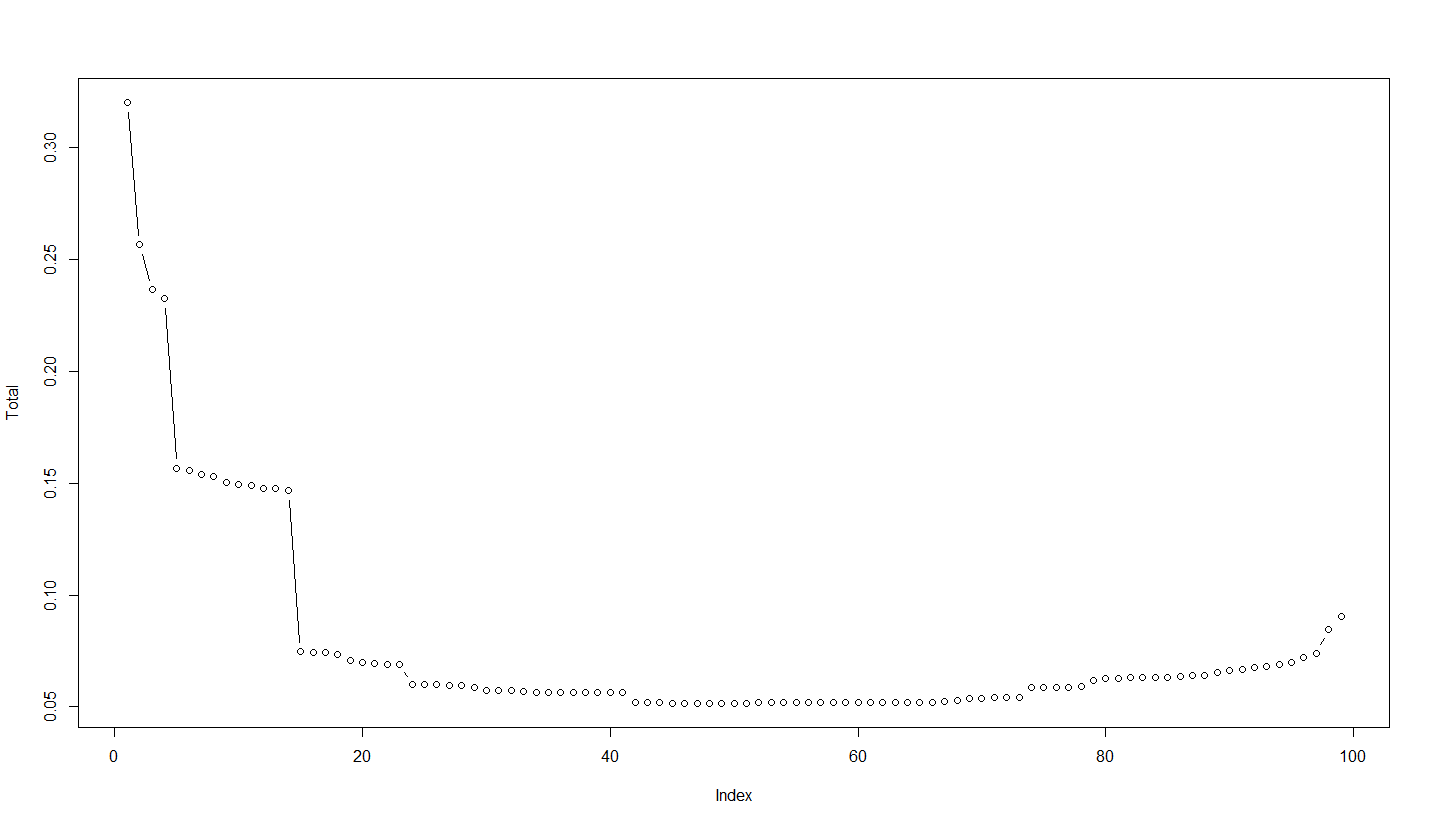
\includegraphics[width=150mm]{alpha.png}
\caption{Optimal value of $\alpha$ to minimize errors}
\end{figure}

\end{enumerate}


 \subsubsection*{Problem 13}

\begin{enumerate}[(a)]
\item Probability mass function:

$$
f(y) = P(Y = y) = 
	\begin{cases}
		\frac{1}{100}, & \text{if}\  Y \in \{1, 2, 3 \dots 100\} \\
		0, & \text{otherwise}
	\end{cases}
$$

Distribution function: $$
F(y) = \sum_{k=1}^{100} P(Y = y_k) = \begin{cases}
		0, & \text{if}\ Y < 1 \\
		\frac{1}{100}, & \text{if}\ 1 \leq  Y < 2 \\
		\frac{2}{100}, & \text{if}\ 2 \leq  Y < 3 \\
				\vdots & \  \\
		\frac{100}{100}, & \text{if}\ 99 \leq  Y < 100 \\
	\end{cases}
$$

Then the mean, ie. the expected value is: $$
\mu = E(Y) = \sum_{y=1}^{100} y f(y) =  \frac{1}{100} \sum_{y=1}^{100} y = \frac{5050}{100} = \textbf{50.5}$$
And the variance is: $$
\sigma^2 =  Var(Y) = E[(Y - \mu)^2] = \sum_{y=1}^{100} (y - \mu)^2 f(y) = \frac{1}{100}  \sum_{y=1}^{100} (y - 50.5)^2 = \frac{3333}{4} =\textbf{ 833.25}
$$

\item Probability mass function:

$$
f(x) = P(X = x) = \frac{{100-x \choose 5}}{{100 \choose 5}} 
$$

Distribution function: $$
F(x) = \sum_{k=1}^{100} P(X = x_k) = \sum_{k=1}^{x} \frac{{100-x \choose 5}}{{100 \choose 5}} 
$$ 

Mean\footnote{I did these calculations with the HP-50g, not in R, hence the fractions}: $$
\mu = E(X) = \sum_{x=1}^{100}  f(X) =  \sum_{x=1}^{100}  \frac{{100-x \choose 5}}{{100 \choose 5}} = \frac{95}{6} = \textbf{15.833}
$$ 

Variance: $$
\sigma^2 = Var(X) = E[(X - \mu)^2] = \sum_{x=1}^{100} (x - \mu)^2 f(x) = \sum_{x=1}^{100} \left( x-\frac{95}{6} \right)^2  \frac{{100-x \choose 5}}{{100 \choose 5}} = \frac{3526115}{1512} = \textbf{2332.08}
$$ 

The variance seems incorrect to me, as it implies a standard deviation of 48.29 but I can't identify my error at the moment.

\end{enumerate} 


\begin{table}[ht!]
\centering
\begin{tabular}{l|cc}
\toprule
& \textbf{Mean} & \textbf{Variance} \\
\midrule
\textbf{(a)} & 50.5 & 833.25 \\
\textbf{(b)} & 15.833 & 2332.08 \\
\toprule
\end{tabular}
\end{table}


 \subsubsection*{Problem 14}
 
 
 The probability that the two-engine plane crashes is the probability that two out of two engines fail.  
 $$ P_{2e} =  p^2  $$
The probability that the four-engine plane crashes is the probability that three or four out of four engines fail.

1. The probability that four engines fail is $p^4$. 

2. The probability that exactly three engines fail is the probability that 3 engines fail and 1 engine doesn't fail, $p^3(1-p)^1$. But since this can happen four different ways, depending on which engine does not fail, the probability is $4(1-p)p^3$.
$$ P_{4e} =  p^4 + 4(1-p)p^3$$
Setting $P_{4e} = P_{2e}$ equal, we can solve for the value of $p$ at the intersection points. 
$$ p^2=  p^4 + 4(1-p)p^3 \rightarrow p=0, p=1, p=\frac{1}{3}$$
Plotting the functions in R:
\begin{figure}[H]
\centering
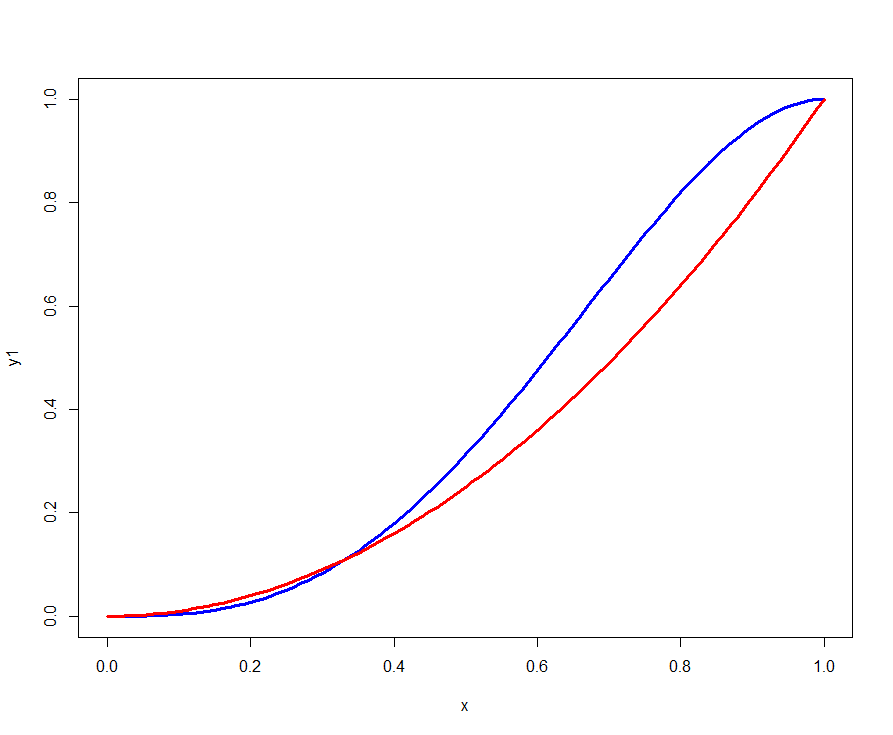
\includegraphics[width=100mm]{EnginesFull.png}
\caption{Four-Engine Plane Failure (Blue) vs. Two-Engine Plane Failure (Red)}
\end{figure}

Since we are interested in the range between 0 and 1, we can see that we would \textit{prefer} the two-engine plane for $\mathbf{1 > p > \frac{1}{3}}$. 

 \subsubsection*{Problem 15}

\begin{enumerate}[(a)]

\item The distribution is a function of the number of right-turns the pinball takes. If the pinball takes 0 right turns, it will be in the 0th position. If it takes 1 right turn, it will be in the 1st position, and so on. 

The probability it will be in cell 0 and 4 is the probability that there are all right-turns or all left-turns over the four possible times to switch: $$ \left( \frac{1}{2} \right)^4 = \frac{1}{16} = 0.0625$$

The probability it will be in cell 1 or 3 is the probability that there are 1 right-turn or left-turn over the four possible times to switch, so the probability is one-in-four: $$ \frac{1}{4} = 0.25 $$

Since there is only cell 2 left, the probability it will be in cell 2 is the probability is the remaining probability: $$  1 - 2(0.0625) - 2(0.25) = 0.375 $$

\item \textbf{Code}: 

\scriptsize 
\begin{verbatim}
from random import randint

def choice():
    return randint(0,1)

def sequence(n):
    return [choice() for i in range(n)]

def position(arr):
    return arr.count(1)

def frequencies(cells):
    counter = [0]*cells

    for i in range(N):
        pos = position(sequence(cells - 1))
        counter[pos] += 1

    return counter 

N = 1000

for i, c in enumerate(frequencies(5)):
    print(i, round(c/N*100,4))
\end{verbatim}
\normalsize

\textbf{Results:}
 
\begin{table}[ht!]
\centering
\begin{tabular}{cccc}
\toprule
\textbf{Cell} & \textbf{Simulation} & \textbf{Theoretical} & \textbf{\% Difference} \\
\midrule
0  &  0.066  &  0.0625  &  5.6 \\
1  &  0.262  &  0.25  &  4.8 \\
2  &  0.354  &  0.375  &  5.6 \\
3  &  0.253  &  0.25  &  1.2 \\
4  &  0.065  &  0.0625  &  4.0 \\
\toprule
\end{tabular}
\end{table}

The simulation results mostly complement the theoretical values, however they would be more accurate if I ran more than 1000 simulations.

\item This distribution is a binomial distribution, that is for each cell $k$, the probability is:

$$ P(k) = {n \choose k} p^k (1-p)^{n-k} $$

Since there is an equal probability of going left or right, then $p=0.5$. Since there are 100 cells, then $n=100$. So for our pinball board, the probability of landing on cell $k$ is:

$$ P(k) = {100 \choose k} 0.5^k (1 - 0.5)^{100-k}  = \frac{100!}{(100-k)! k!} 0.5^k 0.5^{100-k} = \frac{(100!) 0.5^{100}}{(100-k)! k!} $$

See Table 2 for calculated probabilities of landing in cells 0 through 100.


\item I ran the experiment using the above functions in section (b) with the updated parameters. I also calculated the theoretical value from section (c) and calculated the percent difference to compare between the simulated and theoretical values:

\scriptsize
\begin{verbatim}
p = 0.5
n = 100
for k, c in enumerate(frequencies(n)):
    theorical = factorial(n)/(factorial(n-k)*factorial(k))*(p**k)*((1-p)**(n-k))
    print(k, " & ", c/N, " & ", theorical, " & ", round(100*abs(theorical-c/N)/theorical,6), r"\\")
\end{verbatim}
\normalsize




\begin{table}[ht!]
\label{PinboardTable100}
\caption{Pinboard Cell Distribution Theoretical and Simulated}
\tiny
\begin{minipage}{0.5\textwidth}
\begin{tabular}{ccll}
\toprule
\textbf{Cell} & \textbf{Simulation} & \textbf{Theoretical} & \textbf{\% Difference} \\
\midrule
0  &  0.0  &  7.888609052210118e-31  &  100.0 \\
1  &  0.0  &  7.888609052210118e-29  &  100.0 \\
2  &  0.0  &  3.9048614808440084e-27  &  100.0 \\
3  &  0.0  &  1.275588083742376e-25  &  100.0 \\
4  &  0.0  &  3.093301103075262e-24  &  100.0 \\
5  &  0.0  &  5.939138117904503e-23  &  100.0 \\
6  &  0.0  &  9.403635353348797e-22  &  100.0 \\
7  &  0.0  &  1.2627738903068384e-20  &  100.0 \\
8  &  0.0  &  1.4679746474816996e-19  &  100.0 \\
9  &  0.0  &  1.5005963063146263e-18  &  100.0 \\
10  &  0.0  &  1.3655426387463099e-17  &  100.0 \\
11  &  0.0  &  1.1172621589742536e-16  &  100.0 \\
12  &  0.0  &  8.286361012392381e-16  &  100.0 \\
13  &  0.0  &  5.609228993004073e-15  &  100.0 \\
14  &  0.0  &  3.4857351599382454e-14  &  100.0 \\
15  &  0.0  &  1.998488158364594e-13  &  100.0 \\
16  &  0.0  &  1.0616968341311906e-12  &  100.0 \\
17  &  0.0  &  5.246031415707059e-12  &  100.0 \\
18  &  0.0  &  2.4190033750204773e-11  &  100.0 \\
19  &  0.0  &  1.0439909302719954e-10  &  100.0 \\
20  &  0.0  &  4.2281632676015815e-10  &  100.0 \\
21  &  0.0  &  1.6107288638482216e-09  &  100.0 \\
22  &  0.0  &  5.78398092018225e-09  &  100.0 \\
23  &  0.0  &  1.9615239642357197e-08  &  100.0 \\
24  &  0.0  &  6.2932227185896e-08  &  100.0 \\
25  &  0.0  &  1.9131397064512386e-07  &  100.0 \\
26  &  0.0  &  5.518672230147804e-07  &  100.0 \\
27  &  0.0  &  1.5125249815960647e-06  &  100.0 \\
28  &  0.0  &  3.9433687020183116e-06  &  100.0 \\
29  &  0.0  &  9.790432639493739e-06  &  100.0 \\
30  &  0.0  &  2.3170690580135184e-05  &  100.0 \\
31  &  0.0  &  5.232091421320847e-05  &  100.0 \\
32  &  0.0  &  0.00011281697127223077  &  100.0 \\
33  &  0.0  &  0.00023247133474277857  &  100.0 \\
34  &  0.001  &  0.00045810527728724014  &  118.290434 \\
35  &  0.002  &  0.0008638556657416528  &  131.520158 \\
36  &  0.002  &  0.0015597393964779842  &  28.226549 \\
37  &  0.002  &  0.0026979276047186754  &  25.869026 \\
38  &  0.003  &  0.00447287997624412  &  32.929119 \\
39  &  0.006  &  0.00711073226992655  &  15.620505 \\
40  &  0.018  &  0.010843866711637987  &  65.99245 \\
41  &  0.015  &  0.015869073236543397  &  5.476522 \\
42  &  0.028  &  0.022292269546572867  &  25.60408 \\
43  &  0.03  &  0.030068642644214563  &  0.228286 \\
44  &  0.039  &  0.03895255978909614  &  0.12179 \\
45  &  0.047  &  0.048474296626430755  &  3.041399 \\
46  &  0.069  &  0.05795839814029764  &  19.050909 \\
47  &  0.077  &  0.06659049999098027  &  15.63211 \\
48  &  0.071  &  0.07352701040670738  &  3.436846 \\
49  &  0.072  &  0.07802866410507722  &  7.726217 \\
\vdots & \vdots & \vdots & \vdots \\
\toprule
\end{tabular}

\end{minipage} \hfill
\begin{minipage}{0.5\textwidth}

\tiny
\begin{tabular}{ccll}
\toprule
\textbf{Cell} & \textbf{Simulation} & \textbf{Theoretical} & \textbf{\% Difference} \\
\midrule
\vdots & \vdots & \vdots & \vdots \\
50  &  0.086  &  0.07958923738717877  &  8.054811 \\
51  &  0.091  &  0.07802866410507722  &  16.623809 \\
52  &  0.081  &  0.07352701040670738  &  10.163598 \\
53  &  0.054  &  0.06659049999098027  &  18.907352 \\
54  &  0.049  &  0.05795839814029764  &  15.456601 \\
55  &  0.048  &  0.048474296626430755  &  0.97845 \\
56  &  0.037  &  0.03895255978909614  &  5.012661 \\
57  &  0.019  &  0.030068642644214563  &  36.811248 \\
58  &  0.012  &  0.022292269546572867  &  46.16968 \\
59  &  0.013  &  0.015869073236543397  &  18.079652 \\
60  &  0.009  &  0.010843866711637987  &  17.003775 \\
61  &  0.006  &  0.00711073226992655  &  15.620505 \\
62  &  0.01  &  0.00447287997624412  &  123.569603 \\
63  &  0.001  &  0.0026979276047186754  &  62.934513 \\
64  &  0.001  &  0.0015597393964779842  &  35.886726 \\
65  &  0.001  &  0.0008638556657416528  &  15.760079 \\
66  &  0.0  &  0.00045810527728724014  &  100.0 \\
67  &  0.0  &  0.00023247133474277857  &  100.0 \\
68  &  0.0  &  0.00011281697127223077  &  100.0 \\
69  &  0.0  &  5.232091421320847e-05  &  100.0 \\
70  &  0.0  &  2.3170690580135184e-05  &  100.0 \\
71  &  0.0  &  9.790432639493739e-06  &  100.0 \\
72  &  0.0  &  3.9433687020183116e-06  &  100.0 \\
73  &  0.0  &  1.5125249815960647e-06  &  100.0 \\
74  &  0.0  &  5.518672230147804e-07  &  100.0 \\
75  &  0.0  &  1.9131397064512386e-07  &  100.0 \\
76  &  0.0  &  6.2932227185896e-08  &  100.0 \\
77  &  0.0  &  1.9615239642357197e-08  &  100.0 \\
78  &  0.0  &  5.78398092018225e-09  &  100.0 \\
79  &  0.0  &  1.6107288638482216e-09  &  100.0 \\
80  &  0.0  &  4.2281632676015815e-10  &  100.0 \\
81  &  0.0  &  1.0439909302719954e-10  &  100.0 \\
82  &  0.0  &  2.4190033750204773e-11  &  100.0 \\
83  &  0.0  &  5.246031415707059e-12  &  100.0 \\
84  &  0.0  &  1.0616968341311906e-12  &  100.0 \\
85  &  0.0  &  1.998488158364594e-13  &  100.0 \\
86  &  0.0  &  3.4857351599382454e-14  &  100.0 \\
87  &  0.0  &  5.609228993004073e-15  &  100.0 \\
88  &  0.0  &  8.286361012392381e-16  &  100.0 \\
89  &  0.0  &  1.1172621589742536e-16  &  100.0 \\
90  &  0.0  &  1.3655426387463099e-17  &  100.0 \\
91  &  0.0  &  1.5005963063146263e-18  &  100.0 \\
92  &  0.0  &  1.4679746474816996e-19  &  100.0 \\
93  &  0.0  &  1.2627738903068384e-20  &  100.0 \\
94  &  0.0  &  9.403635353348797e-22  &  100.0 \\
95  &  0.0  &  5.939138117904503e-23  &  100.0 \\
96  &  0.0  &  3.093301103075262e-24  &  100.0 \\
97  &  0.0  &  1.275588083742376e-25  &  100.0 \\
98  &  0.0  &  3.9048614808440084e-27  &  100.0 \\
99  &  0.0  &  7.888609052210118e-29  &  100.0 \\
\toprule
\end{tabular}

\end{minipage}
\end{table}



\item In simulation, we see no distribution in the outermost cells, however in the theoretical probabilities there are of course nonzero probabilities. The more iterations we ran, the more likely our simulation would be to reflect the theoretical distribution.

\end{enumerate}


% bibliography
\clearpage
\doublespacing
\bibliographystyle{apacite}
\bibliography{references}



\end{document}
